\chapter{Auswertung}
Der HMF-Gehalt der Proben wird mit zwei Methoden bestimmt. Diese werden im folgenden Abschnitt vorgestellt, angewandt und miteinander verglichen. Außerdem wird die Genauigkeit der beiden Methoden über die Wiederfindungsrate verglichen.
\section{Kalibrierung}
Zur Bestimmung von HMF wird eine Kalibrierung durchgeführt. Um die Linearität des Messsignals bei verschiedenen Konzentrationen zu gewährleisten, müssen mehrere Kalibrierlösungen vermessen werden. Da ein von 5 bis 300mg/kg großer Bereich abgedeckt werden soll, fiel die Entscheidung auf sechs Messpunkte. Die Konzentrationen der Kalibrierstandards sind in folgender Tabelle \ref{tab:Kalibrierungen} eingetragen:

\begin{table}[htbp]
    \centering
    \caption{Kalibrierungen}
        \begin{tabular}{l|c|c|c}
            Standard & Extinktion & Konzentration in mg/L &  Massenanteil in mg/kg\\
            \hline
            Std 1 & 0,0400 & 1,004 & 5\\
            \hline
            Std 2 & 0,1353 & 3,032 & 15\\
            \hline
            Std 3 & 0,1687 & 5,020 & 25\\
            \hline
            Std 4 & 0,3214 & 10,040 & 50\\
            \hline
            Std 5 & 0,9453 & 30,320 & 152\\
            \hline
            Std 6 & 1,8987 & 60,640 & 303
        \end{tabular}
        \label{tab:Kalibrierungen}
\end{table}

Die angegebenen Gehalte und Konzentrationen beziehen sich auf eine theoretische Probeneinwaage von 10,0g Honig.\\
Trägt man nun die Kalibrierpunkte in einem Diagramm ein, ergibt sich eine Gerade mit der Funktion y=0,0309*x+0,0175 bei einem Bestimmtheitsmaß von 0,9997. Die Kalibriergerade ist im folgenden Diagramm \ref{diag:DiagrammKalibrierung} abgebildet und im Anhang 2 zu finden.

\begin{diagram}[htbp]
    \centering
        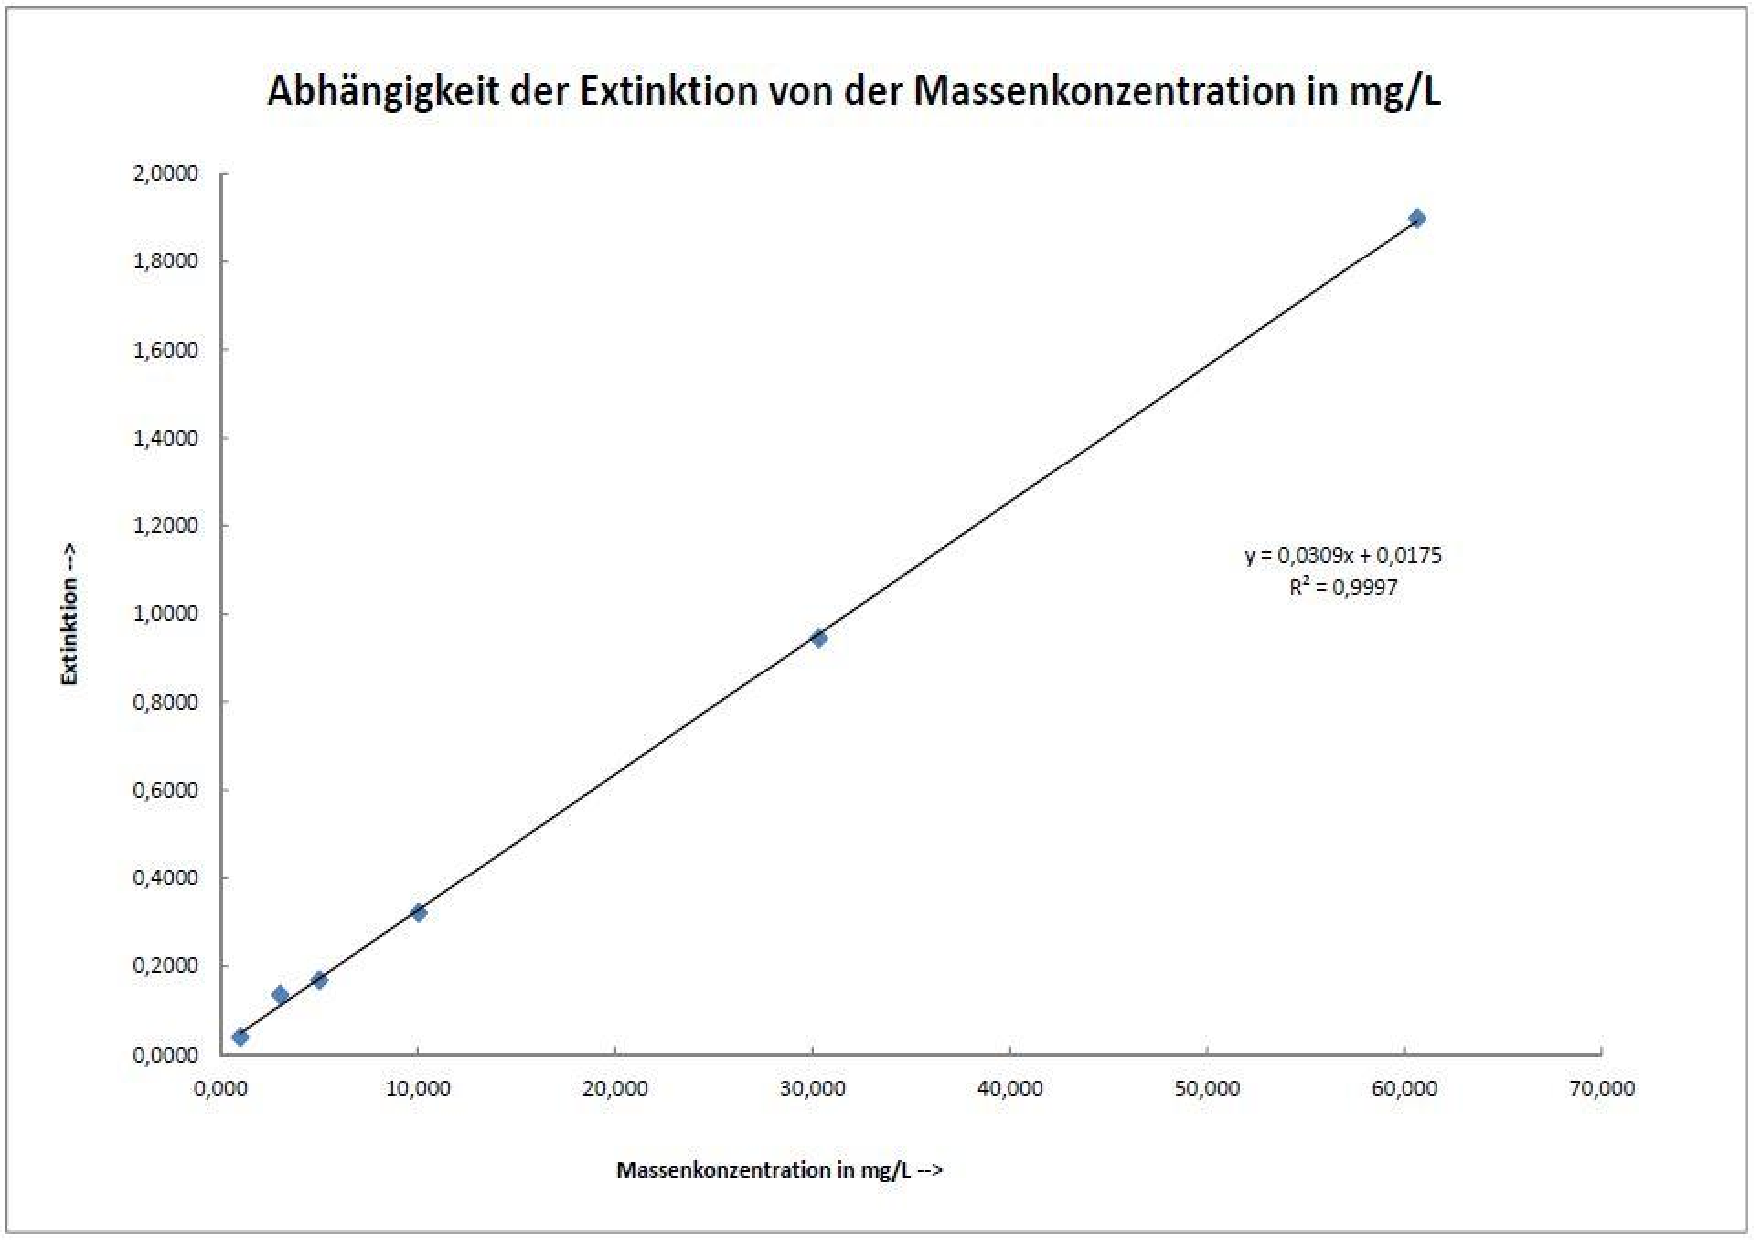
\includegraphics[width=1.00\textwidth]{../Bilder/DiagrammKalibrierung2.pdf}
    \caption{Kalibriergerade}
    \label{diag:DiagrammKalibrierung}
\end{diagram}

\newpage
\section{Quantifizierung mittels Kalibriergerade}
Die durch die Kalibrierung ermittelte Funktion wird zur Bestimmung des Analytgehalts verwendet.
    \begin{eqnarray*}
		y&=&m*x+b\\
    y&=&0,0309*x+0,0175\\
    x&=&\frac{ y-0,0175 }{ 0,0309 }
		\end{eqnarray*}
Beispielrechnung zu Probe 3 (warm):
    \[x=\frac{ 1,9812-0,0175 }{ 0,0309 }\]
    \[x=63,55mg/L\]
Die Massenkonzentration muss nun noch in den Massenanteil umgerechnet werden.
    \[w[mg/kg]=\frac{ \beta*V }{ 1L * m }*1000000\]
    \[w[mg/kg]=\frac{ 0,06355g/L*0,05L }{ 1L * 10,041g }*1000000\]
    \[w[mg/kg]=316mg/kg\]

\newpage
\section{Quantifizierung mittels Festfaktor}
In der Analysevorschrift zur Bestimmung von HMF in Honig ist folgende Formel angegeben:
    \[HMF[mg/kg]=\frac{ E * 1920 }{ m }\]
Hierbei steht E für die Extinktion und m für die Probenmasse. Der Festfaktor 1920 setzt sich zusammen aus dem molaren Extinktionskoeffizienten, der Verdünnung und der Umrechnung in die gewünschte Einheit mg/kg.
    \[Faktor=\frac{ M(HMF)*V }{ \epsilon }*1000000\]

    \[1920=\frac{ 126g/mol * 0,05L }{ 3,28125L/mol }*1000000\]
Beispielrechnung zu Probe 3 (warm):
    \[HMF[mg/kg]=\frac{ 1,9812 * 1920 }{ 10,041g }\]
    \[HMF[mg/kg]=379mg/kg\]

\newpage
\section{Ergebnisse der analysierten Proben}
Alle Proben wurden mit den beiden zur Verfügung stehenden Methoden quantifiziert und die Ergebnisse in der Tabelle \ref{tab:Messergebnisse} festgehalten. Die Messwerte sind in Anhang 3 abgelegt.

\begin{table}[htbp]
    \centering
    \caption{Messergebnisse}
        \begin{tabular}{C{0.1\linewidth}|C{0.24\linewidth}|C{0.14\linewidth}|C{0.23\linewidth}|C{0.25\linewidth}}
            Proben-nummer & Probe & Extinktion & Gehalt HMF über Kalibrierung \newline in mg/kg &  Gehalt HMF über Festfaktor in mg/kg\\
            \hline
            1 & Flotte Biene Frühlingsblütenhonig (kalt) & 0,016 & <5 & <5\\
            \hline
            1 & Flotte Biene Frühlingsblütenhonig (warm) & 1,6041 & 256 & 307\\
            \hline
            2 & Flotte Biene Gebirgsblütenhonig (kalt) & 0,0102 & <5 & <5\\
            \hline
            2 & Flotte Biene Gebirgsblütenhonig (warm) & 1,3184 & 210 & 252\\
            \hline
            3 & Sommerblütenhonig (kalt) & 0,1500 & 20 & 27\\
            \hline
            3 & Sommerblütenhonig (warm) & 1,9812 & 316 & 379\\
            \hline
            4 & Blütenhonig (kalt) & 0,0621 & 7 & 12\\
            \hline
            4 & Blütenhonig (warm) & 1,5500 & 245 & 294\\
            \hline
            5 & Mexico (kalt) & 0,0639 & 8 & 12\\
            \hline
            5 & Mexico (warm) & 1,2237 & 194 & 234\\
            \hline
            6 & Ägäis (kalt) & 0,0871 & 11 & 16\\
            \hline
            6 & Ägäis (warm) & 1,1639 & 185 & 223\\
            \hline
            7 & Waldhonig & 0,0362 & <5 & 7\\
            \hline
            8 & Zuckerrübensirup & n.B. & n.B. & n.B.\\
            \hline
            9 & Winterfutter & 0,0255 & <5 & 5\\
            \hline
            10 & Invertzucker & 1,541 & 249 & 298
        \end{tabular}
    \label{tab:Messergebnisse}
\end{table}

\newpage
\section{Wiederfindungsrate}
Es wurde von Probe 3 (kalt) eine Sechsfachbestimmung durchgeführt und die in Tabelle \ref{tab:Sechsfachbestimmung} festgehaltenen Werte ermittelt:

\begin{table}[htbp]
    \centering
    \caption{Sechsfachbestimmung}
        \begin{tabular}{C{0.1\linewidth}|C{0.24\linewidth}|C{0.14\linewidth}|C{0.23\linewidth}|C{0.25\linewidth}}
            Proben-nummer & Probe & Extinktion & Gehalt HMF über Kalibrierung \newline in mg/kg &  Gehalt HMF über Festfaktor in mg/kg\\
            \hline
            3.1 & Sommerblütenhonig (kalt) & 0,1574 & 22 & 29\\
            \hline
            3.2 & Sommerblütenhonig (kalt) & 0,1676 & 23 & 31\\
            \hline
            3.3 & Sommerblütenhonig (kalt) & 0,1321 & 18 & 25\\
            \hline
            3.4 & Sommerblütenhonig (kalt) & 0,1416 & 19 & 25\\
            \hline
            3.5 & Sommerblütenhonig (kalt) & 0,1662 & 23 & 31\\
            \hline
            3.6 & Sommerblütenhonig (kalt) & 0,1523 & 21 & 28\\
        \end{tabular}
    \label{tab:Sechsfachbestimmung}
\end{table}

Zudem wurde die Probe 3 mit zwei definierten Mengen HMF aufgestockt. Diese sind in Tabelle \ref{tab:Aufstockung} enthalten:

\begin{table}[htbp]
    \centering
    \caption{Aufstockung}
        \begin{tabular}{C{0.1\linewidth}|C{0.24\linewidth}|C{0.14\linewidth}|C{0.23\linewidth}|C{0.25\linewidth}}
            Proben-nummer & Probe & Extinktion & Gehalt HMF über Kalibrierung \newline in mg/kg &  Gehalt HMF über Festfaktor in mg/kg\\
            \hline
            3.7 & Sommerblütenhonig (kalt) & 0,4479 & 66 & 82\\
            \hline
            3.8 & Sommerblütenhonig (kalt) & 0,5734 & 87 & 106\\
        \end{tabular}
    \label{tab:Aufstockung}
\end{table}

Da zur Bestimmung des HMF-Gehalts nur ideale Kalibrierlösungen bzw. der angegebene Festfaktor verwendet wurden, muss der Einfluss der Probenmatrix auf das Analysenergebnis ermittelt werden. Hierzu wird die Wiederfindungsrate anhand einer Aufstockung ermittelt. Die Wiederfindungsrate (WFR) ist der Quotient aus dem Istwert und dem Sollwert der Probe. Zur Berechnung der Wiederfindung wird die folgende Formel verwendet:
    \[WFR=\frac{ Gefundener Gehalt + Istwert }{ Gefundener Gehalt + Sollwert } *100 \]
Als gefundener Gehalt wird der Mittelwert aus der Sechsfachbestimmung der Probe 3 verwendet.
    \[x(Mittelwert)=\frac{ x1+x2...xn }{ n } \]
Die Berechnung des Mittelwertes nach dem in der Vorschrift angegeben Festfaktor:
    \[28mg/kg=\frac{ 29mg/kg+31mg/kg+25mg/kg+25mg/kg+31mg/kg+28mg/kg }{ 6 } \]
Die Berechnung des Mittelwertes nach der erstellten Kalibriergerade:
    \[21mg/kg=\frac{ 22mg/kg+23mg/kg+18mg/kg+19mg/kg+23mg/kg+21mg/kg }{ 6 } \]
Nach dem gemittelten Gehalt muss der aufgestockte Anteil an Analyt berechnet werden. In eine Aufstockung wurden 10ml der Stammlösung 1.1 zugegeben. Das entspricht einer Masse von 0,502 mg. Bezogen auf die Probeneinwaage von 10,483g ergibt sich ein theoretischer Massenanteil von:
    \[w=\frac{ m(Analyt) }{ m(Gesamt) } \]
    \[47,9mg/kg=\frac{ 0,502mg }{ 0,010483kg } \]
In einer zweiten Aufstockung wurden 5ml Stammlösung 2.1 zugegeben, was einer Masse von 0,758mg entspricht. Auch hier wird mit der Einwaage von 10,365g der theoretische Massenanteil berechnet:
    \[73,1mg/kg=\frac{ 0,758mg }{ 0,010365kg } \]
Mit den Mittelwerten und den theoretischen Werten kann die Wiederfindungsrate berechnet werden.\\
Zuerst die erste Aufstockung anhand des Festfaktors:
    \[92,3=\frac{ 28mg/kg + 47,9mg/kg }{ 82mg/kg } *100 \]
Und nach der Kalibriergeraden:
    \[104,4=\frac{ 21mg/kg + 47,9mg/kg }{ 66mg/kg } *100 \]
Anhand der beiden Wiederfindungsraten kann man darauf schließen, dass die Quantifizierung mit der Kalibriergeraden genauere Werte liefert. Zur Kontrolle werden beide Berechnungen noch einmal mit der zweiten Aufstockung durchgeführt.\\
Bestimmung der zweiten Aufstockung nach Festfaktor:
    \[95,4=\frac{ 28mg/kg + 73,1mg/kg }{ 106mg/kg } *100 \]
Bestimmung der zweiten Aufstockung nach Kalibriergeraden:
    \[108,2=\frac{ 21mg/kg + 73,1mg/kg }{ 87mg/kg } *100 \]
Beide Wiederfindungsraten sind nahe 100\%, bei ungefähr gleicher Differenz zum Sollwert. Jedoch findet man mit der Kalibriergeraden tendenziell leicht erhöhte Gehalte an HMF wieder (104,4 und 108,2\%), während man in den Proben weniger HMF findet. Es ist auch bemerkenswert wie gut der angegebene Festfaktor zur Gehaltsbestimmung geeignet ist, obwohl bei seiner Verwendung in keinster Weise kalibriert wird und das verwendete Messgerät damit völlig ignoriert wird. Auch bei der Genauigkeit der Ergebnisse sind beide Methoden vergleichbar.
\subsection{Standardabweichung}
Da die Probe 3 sechs mal bestimmt wurde, wird die Standardabweichung ermittelt. Mit ihr kann eine Aussage über die Streuung der Messergebnisse getroffen werden. In einem ersten Schritt wird der Mittelwert der Sechsfachbestimmung von Probe 3 bestimmt. Dazu kann der Mittelwert aus dem Abschnitt über die Wiederfindungsrate verwendet werden. Exemplarisch wird die Quantifizierung über den Festfaktor verwendet.\\
Mit den Messwerten kann die Varianz $s^{ 2 }$ ermittelt werden:

    \[s^{ 2 }=\frac{ (x_{ 1 }-\bar{x})^{ 2 }+(x_{ 2 }-\bar{x})^{ 2 }+...(x_{ n }-\bar{x})^{ 2 } }{ n-1 }\]
    \[7,40=\frac{ (29-28)^{ 2 }+(31-28)^{ 2 }+(25-28)^{ 2 }+(25-28)^{ 2 }+(31-28)^{ 2 }+(28-28)^{ 2 } }{ 5 }\]

Die Standardabweichung entspricht der Wurzel der Varianz:

    \[s=\sqrt{ 7,40 }\]
    \[s=2,72\]

Die Standardabweichung beträgt 2,72mg/kg. Zur besseren Veranschaulichung kann noch die relative Standardabweichung herangezogen werden:
    \[rel.s=\frac{ s }{ \bar{x} }*100\%\]
    \[rel.s=\frac{ 2,72 }{ 28 }*100\%\]
    \[rel.s=9,7\%\]

Die relative Standardabweichung beträgt somit 9,7\%. In Anbetracht des geringen gemessenen Gehaltes ist dies ein akzeptabler Wert.

\section{Standardaddition}
Da die Probe 3 zweimal mit unterschiedlichen Mengen an HMF aufgestockt wurde, wird zusätzliche eine Quantifizierung über die Standardaddition durchgeführt. So lässt sich auch der Einfluss der nach der Abtrennung noch enthaltenen Probenmatrix eliminieren. Eine Übereinstimmung mit unseren anderen Ergebnissen würde für einen nur unwesentlichen Einfluss der verbliebenen Matrixanteile sprechen. Der Massenanteil mit mehreren Aufstockungen wird berechnet in dem man die Extinktion der Probe (hier die Mittelwerte der sechs Bestimmungen von Probe 3), sowie die Extinktionen der Aufstockungen zur Erstellung eines Diagramms verwendet. Die Probe ohne Aufstockung markiert den Nullpunkt der X-Achse, jede Aufstockung ist auf der X-Achse gemäß ihrer zugesetzten Konzentration aufgetragen. Das nachfolgende Diagramm \ref{diag:Standardaddidtion} verdeutlicht die Auswertung.
\begin{diagram}[htbp]
    \centering
        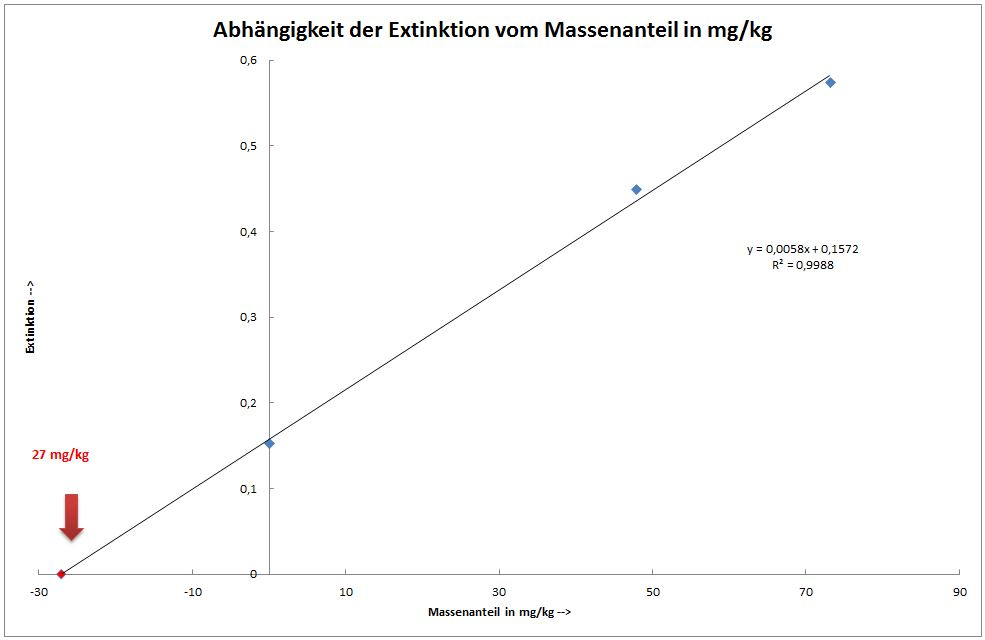
\includegraphics[width=1.00\textwidth]{../Bilder/Standardaddidtion.JPG}
    \caption{Standardaddition}
    \label{diag:Standardaddidtion}
\end{diagram}



Zieht man durch die erhaltenen Punkte eine Gerade und verlängert sie zurück bis sie die X-Achse im negativen Bereich schneidet, kann man an diesem Punkt die Konzentration der Probe graphisch ablesen. Der Gehalt der Probe lässt sich zudem über die lineare Regression der Geraden bestimmen. Sie lautet bei dieser Analyse:
    \[y=0,0058*x+0,1572\]
Setzt man y nun gleich 0 und löst nach x auf erhält man die Konzentration der Probe in mg/kg.
    \[0=0,0058*x+0,1572\]
    \[x=\frac{ -1,572 }{ 0,0058 }   |*-1\]
    \[x=27mg/kg\]
Der über Standardaddition ermittelte Gehalt an HMF in der Probe 3 ist damit 27mg/kg und entspricht somit praktisch dem Gehalt, der mit den anderen Quantifizierungsmethoden ermittelt wurde.
